\documentclass[13pt,a4paper]{article}
\usepackage{a4wide,amssymb,epsfig,latexsym,multicol,array,hhline,fancyhdr}
\usepackage{amsmath}
\usepackage{amsfonts}
\usepackage{lastpage}
\usepackage[lined,boxed,commentsnumbered]{algorithm2e}
\usepackage{enumerate}
\usepackage{color}
\usepackage{graphicx}							% Standard graphics package
\usepackage{array}
\usepackage{tabularx, caption}
\usepackage{multirow}
\usepackage{multicol}
\usepackage{rotating}
\usepackage{graphics}
\usepackage{geometry}
\usepackage{setspace}
\usepackage{subfig}
\usepackage{epsfig}
\usepackage{tikz}
\usetikzlibrary{arrows,snakes,backgrounds}
\usepackage{hyperref}
\hypersetup{urlcolor=blue,linkcolor=black,citecolor=black,colorlinks=true} 
%\usepackage{pstcol} 								% PSTricks with the standard color package

\newtheorem{theorem}{{\bf Theorem}}
\newtheorem{property}{{\bf Property}}
\newtheorem{proposition}{{\bf Proposition}}
\newtheorem{corollary}[proposition]{{\bf Corollary}}
\newtheorem{lemma}[proposition]{{\bf Lemma}}

\AtBeginDocument{\renewcommand*\contentsname{Contents}}
\AtBeginDocument{\renewcommand*\refname{References}}
%\usepackage{fancyhdr}
\setlength{\headheight}{40pt}
\pagestyle{fancy}
\fancyhead{} % clear all header fields
\fancyhead[L]{
	\begin{tabular}{rl}
		\begin{picture}(25,15)(0,0)
			\put(0,-8){
\includegraphics[width=8mm, height=8mm]{hcmut.png}}
			%\put(0,-8){\epsfig{width=10mm,figure=hcmut.eps}}
		\end{picture}&
		%
\includegraphics[width=8mm, height=8mm]{hcmut.png} & %
		\begin{tabular}{l}
			\textbf{\bf \ttfamily University of Technology, Ho Chi Minh City}\\
			\textbf{\bf \ttfamily Faculty of Computer Science and Engineering}
		\end{tabular} 	
	\end{tabular}
}
\fancyhead[R]{
	\begin{tabular}{l}
		\tiny \bf \\
		\tiny \bf 
\end{tabular}  }
\fancyfoot{} % clear all footer fields
\fancyfoot[L]{\scriptsize \ttfamily Lab 8 for Operating Systems year 2020 - 2021}
\fancyfoot[R]{\scriptsize \ttfamily Page {\thepage}/\pageref{LastPage}}
\renewcommand{\headrulewidth}{0.3pt}
\renewcommand{\footrulewidth}{0.3pt}


%%%
\setcounter{secnumdepth}{4}
\setcounter{tocdepth}{3}
\makeatletter
\newcounter {subsubsubsection}[subsubsection]
\renewcommand\thesubsubsubsection{\thesubsubsection .\@alph\c@subsubsubsection}
\newcommand\subsubsubsection{\@startsection{subsubsubsection}{4}{\z@}%
	{-3.25ex\@plus -1ex \@minus -.2ex}%
	{1.5ex \@plus .2ex}%
	{\normalfont\normalsize\bfseries}}
\newcommand*\l@subsubsubsection{\@dottedtocline{3}{10.0em}{4.1em}}
\newcommand*{\subsubsubsectionmark}[1]{}
\makeatother

\begin{document}
	
	\begin{titlepage}
		\begin{center}
			VIETNAM NATIONAL UNIVERSITY, HO CHI MINH CITY \\
			UNIVERSITY OF TECHNOLOGY \\
			FACULTY OF COMPUTER SCIENCE AND ENGINEERING
		\end{center}
		
		\vspace{1cm}
		
		\begin{figure}[h!]
			\begin{center}
				
\includegraphics[width=3cm]{hcmut.png}
			\end{center}
		\end{figure}
		
		\vspace{1cm}
		
		\begin{center}
			\color{blue}
			\begin{tabular}{c}
				\multicolumn{1}{l}{\textbf{\centerline{{\Huge DIGITAL SIGNAL PROCESSING}}}}\\
				~~\\
				\hline
				\\
				\multicolumn{1}{l}{\textbf{\centerline{{\LARGE Report \#08}}}}\\
				\\
				\textbf{{\Huge Lab 08 : Z - Transform}}\\
				\\
				\hline
			\end{tabular}
			\color{blue}
		\end{center}
		\vspace{1cm}
		
		\begin{table}[h]
			\color{blue}
			\begin{tabular}{rrl}
				\hspace{5 cm} & Advisor: & Tran Minh Duc\\
				& Students: & Tran Long Vi - 1814804 \\
			\end{tabular}
			\color{blue}
		\end{table}
		
		\vspace{4 cm}
		\begin{center}
			{\footnotesize\large HO CHI MINH CITY, DECEMBER 2020}
		\end{center}
	\end{titlepage}
	
	
	%\thispagestyle{empty}
	\newpage
	
	
	%%%%%%%%%%%%%%%%%%%%%%%%%%%%%%%%%
	\section{Exercise 1 : Find the all possible signal $x(n)$ that have Z transforms as follows}
		\begin{enumerate}[a)]
			\item $x(z) = \dfrac{1 - 1.5z^{-1}}{1 - 1.5z^{-1} + 0.5z^{-2}}$ \\
				$
					1 - 1.5z^{-1} + 0.5z^{-2} = (1 - \alpha z^{-1})(1 - \beta z^{-1}) \\
					\rightarrow \left\{\begin{array}{l}
						\alpha + \beta = 1.5 \\
						\alpha \cdot \beta = 0.5
					\end{array}\right. \\
					\rightarrow \left\{\begin{array}{l}
						\alpha = 0.5 \\
						\beta = 1
					\end{array}\right. \\ \\
					1 - 1.5z^{-1} = A(1 - z^{-1}) + B(1 - 0.5z^{-1}) \\
					\rightarrow \left\{\begin{array}{c}
						A + B = 1 \\
						0.5A + B = 1.5
					\end{array}\right. \\
					\rightarrow \left\{\begin{array}{l}
						A = -1 \\
						B = 2
					\end{array}\right. \\
					\Rightarrow x(z) = \dfrac{-1}{1 - 0.5z^{-1}} + \dfrac{2}{1 - z^{-1}} \\
					Result: \left\{\begin{array}{lll}
						x(n) = - 0.5^nu(n) + 2u(n), & |z| > 1 \\
						x(n) = - 0.5^nu(n) + 2u(-n - 1), & 0.5 < |z| < 1 \\
						x(n) = - 0.5^nu(-n - 1) + 2u(-n - 1), & |z| < 0.5
					\end{array}\right.
				$ \\
			\item $x(z) = \dfrac{1}{1 - z^{-1} + 0.25z^{-2}}$	\\
				$
					1 - z^{-1} + 0.25z^{-2} = (1 - \alpha z^{-1})(1 - \beta z^{-1}) \\
					\rightarrow \left\{\begin{array}{l}
						\alpha + \beta = 1 \\
						\alpha \cdot \beta = 0.25
					\end{array}\right. \\
					\rightarrow \left\{\begin{array}{l}
						\alpha = 0.5 \\
						\beta = 0.5
					\end{array}\right. \\ \\
					\Rightarrow x(z) = \dfrac{1}{(1 - 0.5z^{-1})^2} \\
					\Rightarrow x(z) = \dfrac{1}{1 - 0.5z^{-1}} + \dfrac{0.5z^{-1}}{(1 - 0.5z^{-1})^2}\\
					Result: \left\{\begin{array}{lll}
						x(n) = 0.5^nu(n) + n \cdot 0.5^nu(n), & |z| > 0.5 \\
						x(n) = -0.5^nu(-n - 1) - n \cdot 0.5^nu(-n - 1), & |z| < 0.5
					\end{array}\right.
				$ \\
			\item $x(z) = \dfrac{1}{3 - 10z^{-1} + 3z^{-2}}$ \\
				$
					3 - 10z^{-1} + 3z^{-2} = 3(1 - \alpha z^{-1})(1 - \beta z^{-1}) \\
					\Leftrightarrow  x(z) = \dfrac{1}{3(1 - \frac{1}{3}z^{-1})(1 - 3z^{-1})} \\
					1 = A(1 - \frac{1}{3}z^{-1}) + B(1 - 3z^{-1}) \\
					\rightarrow \left\{\begin{array}{c}
						\frac{1}{3}A + 3B = 0 \\
						A + B = 1
					\end{array}\right. \\
					\rightarrow \left\{\begin{array}{l}
						A = \frac{9}{8} \\
						B = -\frac{1}{8}
					\end{array}\right. \\
					\Rightarrow x(z) = \dfrac{\frac{-1}{24}}{1 - \frac{1}{3}z^{-1}} + \dfrac{\frac{3}{8}}{1 - 3z^{-1}} \\
					Result: \left\{\begin{array}{lll}
						x(n) = \frac{-1}{24} \cdot (\frac{1}{3})^nu(n) + \frac{3}{8} \cdot 3^nu(n), & |z| > 3 \\
						x(n) = \frac{-1}{24} \cdot (\frac{1}{3})^nu(n) - \frac{3}{8} \cdot 3^nu(-n - 1), & \frac{1}{3} < |z| < 3\\
						x(n) =\frac{-1}{24} \cdot (\frac{1}{3})^nu(-n - 1) - \frac{3}{8} \cdot 3^nu(-n - 1), & |z| < \frac{1}{3}
					\end{array}\right.
				$ \\
			\item $x(z) = \dfrac{1}{2 - 3z^{-1} + 1z^{-2}}$ \\
				$
					\Leftrightarrow x(z) = \dfrac{1}{2 - 3z^{-1} + 1z^{-2}} = \dfrac{1}z{(1 - 2z^{-1})(1 - z^{-1})} \\
					1 = A(1 - z^{-1}) + B(1 - 2z^{-1}) \\
					\rightarrow \left\{\begin{array}{c}
						A + 2B = 0 \\
						A + B = 1
					\end{array}\right. \\
					\rightarrow \left\{\begin{array}{l}
						A = 2 \\
						B = -1
					\end{array}\right. \\
					\Rightarrow x(z) = \dfrac{2}{1 - 2z^{-1}} + \dfrac{-1}{1 - z^{-1}} \\
					Result: \left\{\begin{array}{lll}
						x(n) = 2^{n+1}u(n) - u(n), & |z| > 2 \\
						x(n) = 2^{n+1}u(n) + u(-n - 1), & 1 < |z| < 2\\
						x(n) = 2^{n+1}u(-n - 1) - u(-n - 1), & |z| < 1
					\end{array}\right.
				$ \\
			\item $x(z) = \dfrac{1 + 2z^{-1} + z^{-2}}{1 + 4z^{-1} + 4z^{-2}}$ \\
				$
					\Leftrightarrow x(z) = \dfrac{1 + 2z^{-1} + z^{-2}}{1 + 4z^{-1} + 4z^{-2}} = \dfrac{(1 + z^{-1})^2}{4(1 + \frac{1}{2}z^{-1})^2} = \left(\frac{1}{2} \cdot \dfrac{1 + z^{-1}}{1 + \frac{1}{2}z^{-1}}\right)^2 \\
					1 + z^{-1} = A + B(1 + \frac{1}{2}z^{-1}) \\
					\rightarrow \left\{\begin{array}{c}
						\frac{1}{2}B = 1 \\
						A + B = 1
					\end{array}\right. \\
					\rightarrow \left\{\begin{array}{l}
						A = -1 \\
						B = 2
					\end{array}\right. \\
					\Rightarrow x(z) = \left(1 - \dfrac{\frac{1}{2}}{1 + \frac{1}{2}z^{-1}}\right)^2 \\
					\Leftrightarrow x(z) = \frac{1}{4} \cdot \dfrac{1}{(1 + \frac{1}{2}z^{-1})^2} - \dfrac{1}{1 + \frac{1}{2}z^{-1}} + 1 \\
					\Leftrightarrow x(z) = \frac{1}{4} \cdot \left(\dfrac{1}{1 + \frac{1}{2}z^{-1}} - \dfrac{\frac{1}{2}z^{-1}}{(1 + \frac{1}{2}z^{-1})^2}\right) - \dfrac{1}{1 + \frac{1}{2}z^{-1}} + 1 \\
					\Leftrightarrow x(z) = \dfrac{\frac{1}{4}}{1 + \frac{1}{2}z^{-1}} - \dfrac{\frac{1}{8}z^{-1}}{(1 + \frac{1}{2}z^{-1})^2} - \dfrac{1}{1 + \frac{1}{2}z^{-1}} + 1 \\ \\
					Result: \left\{\begin{array}{lll}
						x(n) = \frac{1}{4} \cdot (\frac{1}{2})^nu(n) - \frac{1}{4} \cdot n \cdot (\frac{1}{2})^nu(n) - (\frac{1}{2})^nu(n) + \delta(n), & |z| > \frac{1}{2} \\ \\
						x(n) = -\frac{1}{4} \cdot (\frac{1}{2})^nu(-n - 1) + \frac{1}{4} \cdot n \cdot (\frac{1}{2})^nu(-n - 1) + (\frac{1}{2})^nu(-n - 1) + \delta(n), & |z| < \frac{1}{2}
					\end{array}\right.
				$\\
			\item $x(z) = \dfrac{2z^2 - 12z}{(z - 0.3)(z + 0.2)(z - 3)}$ \\
				$
					\Leftrightarrow x(z) = 2\left(\dfrac{z^2 - 6z}{z^3(1 - 0.3z^{-1})(1 + 0.2z^{-1})(1 - 3z^{-1})}\right) = 2\left(\dfrac{z^{-1} - 6z^{-2}}{(1 - 0.3z^{-1})(1 + 0.2z^{-1})(1 - 3z^{-1})}\right) \\
					z^{-1} - 6z^{-2} = A(1 - 0.3z^{-1})(1 + 0.2z^{-1}) + B(1 + 0.2z^{-1})(1 - 3z^{-1}) + C(1 - 0.3z^{-1})(1 - 3z^{-1}) \\
					\Leftrightarrow z^{-1} - 6z^{-2} = A(1 - 0.1z^{-1} - 0.06z^{-2}) + B(1 - 2.8z^{-1} - 0.6z^{-2}) + C(1 - 3.3z^{-1} + 0.9z^{-2}) \\
					\rightarrow \left\{\begin{array}{l}
						A + B + C = 0 \\
						0.1A + 2.8B + 3.3C = -1 \\
						0.06A + 0.6B - 0.9C = 6
					\end{array}\right. \\
					\rightarrow \left\{\begin{array}{l}
						A = -\frac{25}{72} \\
						B = \frac{38}{9} \\
						C = -\frac{31}{8}
					\end{array}\right. \\
					\Leftrightarrow x(z) = \dfrac{\frac{76}{9}}{1 - 0.3z^{-1}} + \dfrac{-\frac{31}{4}}{1 + 0.2z^{-1}} + \dfrac{-\frac{25}{36}}{1 - 3z^{-1}} \\ \\
					Result: \left\{\begin{array}{lll}
						x(n) = \frac{76}{9} \cdot 0.3^nu(n) - \frac{31}{4} \cdot (-0.2)^nu(n) - \frac{25}{36} \cdot 3^nu(n),& |z| > 3 \\ \\
						x(n) = \frac{76}{9} \cdot 0.3^nu(n) - \frac{31}{4} \cdot (-0.2)^nu(n) + \frac{25}{36} \cdot 3^nu(-n - 1),& 0.3 < |z| < 3 \\ \\ 
						x(n) = \frac{76}{9} \cdot 0.3^nu(n) + \frac{31}{4} \cdot (-0.2)^nu(-n - 1) + \frac{25}{36} \cdot 3^nu(-n - 1),& 0.2 < |z| < 0.3 \\ \\
						x(n) = -\frac{76}{9} \cdot 0.3^nu(-n - 1) + \frac{31}{4} \cdot (-0.2)^nu(-n - 1) + \frac{25}{36} \cdot 3^nu(-n - 1),& |z| < 0.2
					\end{array}\right.
				$
		\end{enumerate}
	\section{Exercise 2 : Compute the convolution $x(n) = x_1(n) * x_2(n)$ using $Z$ and Inverse $Z$ transform, where:}
		\begin{enumerate}[a)]
			\item $x_1(n) = \{1^{\uparrow}, 1, 1, 1, 1\}, x_2(n) = \{1^{\uparrow}, 1, 1, 1\}$ \\
				$
					\Rightarrow x_1(z) = 1 + z^{-1} + z^{-2} + z^{-3} + z^{-4},\qquad x_2(z) = 1 + z^{-1} + z^{-2} + z^{-3} \\
					x(n) = x_1(n) * x_2(n) \longrightarrow x(z) = x_1(z) \cdot x_2(z) \\
					\Leftrightarrow x(z) = (1 + z^{-1} + z^{-2} + z^{-3} + z^{-4})(1 + z^{-1} + z^{-2} + z^{-3}) \\
					\Leftrightarrow x(z) = 1 + 2z^{-1} + 3z^{-2} + 4z^{-3} + 3z^{-4} + 2z^{-5} + z^{-6} \\
					Result: x(n) = x_1(n) * x_2(n) = Z^{-1}[x(z)] = \{1^{\uparrow}, 2, 3, 4, 3, 2, 1\} \\
				$
			\item $x_1(n) = \{1^{\uparrow}, 2, 3, 4, 5\}, x_2(n) = \{1^{\uparrow}, 1, 1\}$ \\
				$
					\Rightarrow x_1(z) = 1 + 2z^{-1} + 3z^{-2} + 4z^{-3} + 5z^{-4},\qquad x_2(z) = 1 + z^{-1} + z^{-2} \\
					x(n) = x_1(n) * x_2(n) \longrightarrow x(z) = x_1(z) \cdot x_2(z) \\
					\Leftrightarrow x(z) = (1 + 2z^{-1} + 3z^{-2} + 4z^{-3} + 5z^{-4})(1 + z^{-1} + z^{-2}) \\
					\Leftrightarrow x(z) = 1 + 3z^{-1} + 6z^{-2} + 9z^{-3} + 12z^{-4} + 9z^{-5} + 5z^{-6} \\
					Result: x(n) = x_1(n) * x_2(n) = Z^{-1}[x(z)] = \{1^{\uparrow}, 3, 6, 9, 12, 9, 5\} \\
				$
			\item $x_1(n) = \left(\frac{1}{5}\right)^nu(n), x_2(n) = 2^nu(n)$ \\
				$
					\Rightarrow \left\{\begin{array}{lll}
						x_1(z) = \dfrac{1}{1 - 0.2z^{-1}},& |z| > 0.2
						x_2(z) = \dfrac{1}{1 - 2z^{-1}},& |z| > 2 \\
						0.2A + 2B = 0
					\end{array}\right. \\
					x(n) = x_1(n) * x_2(n) \longrightarrow x(z) = x_1(z) \cdot x_2(z) \\
					\Leftrightarrow x(z) = \dfrac{1}{(1 - 0.2z^{-1})(1 - 2z^{-1})} \\
					1 = A(1 - 0.2z^{-1}) + B(1 - 2z^{-1}) \\
					\rightarrow \left\{\begin{array}{c}
						A + B = 1 \\
						0.2A + 2B = 0
					\end{array}\right. \\
					\rightarrow \left\{\begin{array}{l}
						A = \frac{10}{9} \\
						B = -\frac{1}{9}
					\end{array}\right. \\
					\Leftrightarrow x(z) = \dfrac{-\frac{1}{9}}{1 - 0.2z^{-1}} + \dfrac{\frac{10}{9}}{1 - 2z^{-1}} \\
					Result: x(n) = -\frac{1}{9} \cdot 0.2^nu(n) + \frac{10}{9} \cdot 2^nu(n),\qquad |z| > 2 \\
				$
			\item $x_1(n) = nu(n), x_2(n) = 2^nu(n - 1)$ \\
				$
					\Rightarrow \left\{\begin{array}{lll}
						x_1(z) = \dfrac{z^{-1}}{(1 - z^{-1})^2},& |z| > 1 \\
						x_2(z) = \dfrac{2z^{-1}}{1 - 2z^{-1}},& |z| > 2
					\end{array}\right. \\ \\
					x(n) = x_1(n) * x_2(n) \longrightarrow x(z) = x_1(z) \cdot x_2(z) \\
					\Leftrightarrow x(z) = \dfrac{2z^{-2}}{(1 - z^{-1})^2(1 - 2z^{-1})} \\ \\
					2z^{-2} = A(1 - z^{-1})^2 + B(1 - 2z^{-1}) \\
					\Rightarrow \left\{\begin{array}{lll}
						A + B = 0 \\
						A = 2
					\end{array}\right. \\
					\Rightarrow \left\{\begin{array}{lll}
						A = 2 \\
						B = -2
					\end{array}\right. \\
					\Leftrightarrow x(z) = \dfrac{-2}{(1 - z^{-1})^2} + \dfrac{2}{1 - 2z^{-1}} \\
					\Leftrightarrow x(z) = \dfrac{-2}{1 - z^{-1}} - \dfrac{2z^{-1}}{(1 - z^{-1})^2} + \dfrac{2}{1 - 2z^{-1}} \\
					Result: x(n) = -2 \cdot u(n) - 2 \cdot nu(n) + 2^nu(n), \qquad |z| > 2
				$
		\end{enumerate}
	\section{Exercise 3 : Given an LTI system represented by the input - output description equation}
		\begin{enumerate}[a)]
			\item Draw corresponding block diagram \\
				$Y(z) = 0.7z^{-1}Y(z) + X(z)$ 
				\begin{figure}[h!]
					\begin{center}
						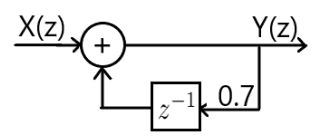
\includegraphics[width=7cm]{cau3.png}
						\caption{Block diagram}
					\end{center}
				\end{figure}
			\item Determine $h(n)$ using Z and inverse Z transforms. \\
				$
					y(n) = 0.7y(n - 1) + x(n) \\
					\Rightarrow Y(z)(1 - 0.7z^{-1}) = X(z) \\ \\
					h(z) = \dfrac{Y(z)}{X(z)} = \dfrac{1}{1 - 0.7z^{-1}} \\
					\Rightarrow \left\{\begin{array}{ll}
						h(n) = 0.7^nu(n),& |z| > 0.7 \\
 						h(n) = 0.7^nu(-n - 1),& |z| < 0.7
					\end{array}\right. \\
				$
			\item Determine $y(n)$ when $x(n) = u(n)$ \\
				$
					When\ x(n) = u(n): y(n) = 0.7y(n - 1) + u(n)\\
					\Rightarrow Y(z)(1 - 0.7z^{-1}) = \dfrac{1}{1 - z^{-1}} \\
					\Rightarrow Y(z) = \dfrac{1}{(1 - 0.7z^{-1})(1 - z^{-1})}, \qquad |z| > 1 \\ 
					1 = A(1 - 0.7z^{-1}) + B(1 - z^{-1}) \\
					\rightarrow \left\{\begin{array}{c}
						A + B = 1 \\
						0.7A + B = 0
					\end{array}\right. \\
					\rightarrow \left\{\begin{array}{l}
						A = \frac{10}{3} \\
						B = -\frac{7}{3}
					\end{array}\right. \\
					\Leftrightarrow Y(z) = \dfrac{-\frac{7}{3}}{(1 - 0.7z^{-1})} + \dfrac{\frac{10}{3}}{(1 - z^{-1})} \\ \\
					\Rightarrow y(n) = -\frac{7}{3} \cdot 0.7^nu(n) + \frac{10}{3} \cdot u(n), \qquad |z| > 1 \\
				$
		\end{enumerate}
	\section{Exercise 4 : Given an LTI system represented by the input - output description equation}
		\begin{enumerate}[a)]
			\item Draw corresponding block diagram \\
				$Y(z) = 0.5z^{-1}Y(z) + X(z) + z^{-1}X(z)$ 
				\begin{figure}[h!]
					\begin{center}
						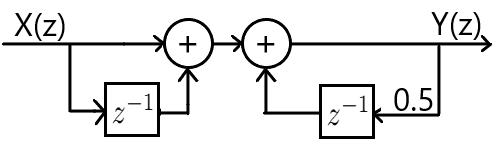
\includegraphics[width=7cm]{cau4.png}
						\caption{Block diagram}
					\end{center}
				\end{figure}			
			\item Determine $h(n)$ using Z and inverse Z transforms. \\
				$
					y(n) = 0.5y(n - 1) + x(n) + x(n - 1) \\
					\Rightarrow Y(z)(1 - 0.5z^{-1}) = X(z)(1 + z^{-1})	\\ \\
					h(z) = \dfrac{Y(z)}{X(z)} = \dfrac{1 + z^{-1}}{1 - 0.5z^{-1}} = \dfrac{1}{1 - 0.5z^{-1}} + 2\dfrac{0.5z^{-1}}{1 - 0.5z^{-1}} \\
					\Rightarrow \left\{\begin{array}{ll}
						h(n) = 0.5^nu(n) + 2 \cdot 0.5^nu(n - 1),& |z| > 0.5 \\
						h(n) = 0.5^nu(-n - 1) + 2 \cdot 0.5^nu(-n),& |z| < 0.5
					\end{array}\right. \\
				$
			\item Determine $y(n)$ when $x(n) = 2^nu(n)$ \\
				$
					When\ x(n) = 2^nu(n): \\
					Y(z)(1 - 0.5z^{-1}) = X(z)(1 + z^{-1}) \\
					\Leftrightarrow Y(z) = \dfrac{1 + z^{-1}}{1 - 0.5z^{-1}} \cdot \dfrac{1}{1 - 2z^{-1}}, \qquad |z| > 2 \\ \\
					1 + z^{-1} = A(1 - 0.5z^{-1}) + B(1 - 2z^{-1}) \\
					\rightarrow \left\{\begin{array}{c}
						A + B = 1 \\
						0.5A + 2B = 1
					\end{array}\right. \\
					\rightarrow \left\{\begin{array}{l}
						A = \frac{2}{3} \\
						B = \frac{1}{3}
					\end{array}\right. \\
					\Leftrightarrow Y(z) = \dfrac{\frac{1}{3}}{(1 - 0.5z^{-1})} + \dfrac{\frac{2}{3}}{(1 - 2z^{-1})} \\ \\
					\Rightarrow y(n) = \frac{1}{3} \cdot 0.5^nu(n) + \frac{2}{3} \cdot 2^nu(n), \qquad |z| > 2 \\
				$
		\end{enumerate}
	\section{Exercise 5 : Use SciLab to find $h(n)$ where}
		\begin{enumerate}[a)]
			\item $H(z) = \dfrac{z^{-2}}{1 - 3z^{-1} + 2z^{-2}}, \qquad |z| > 2$ \\
				$Replace\ s = z^{-1} \Rightarrow H(s) = \dfrac{s^2}{1 - 3s^1 + 2s^2}$ \\
				after using Scilab like below,
				\begin{figure}[h!]
					\begin{center}
						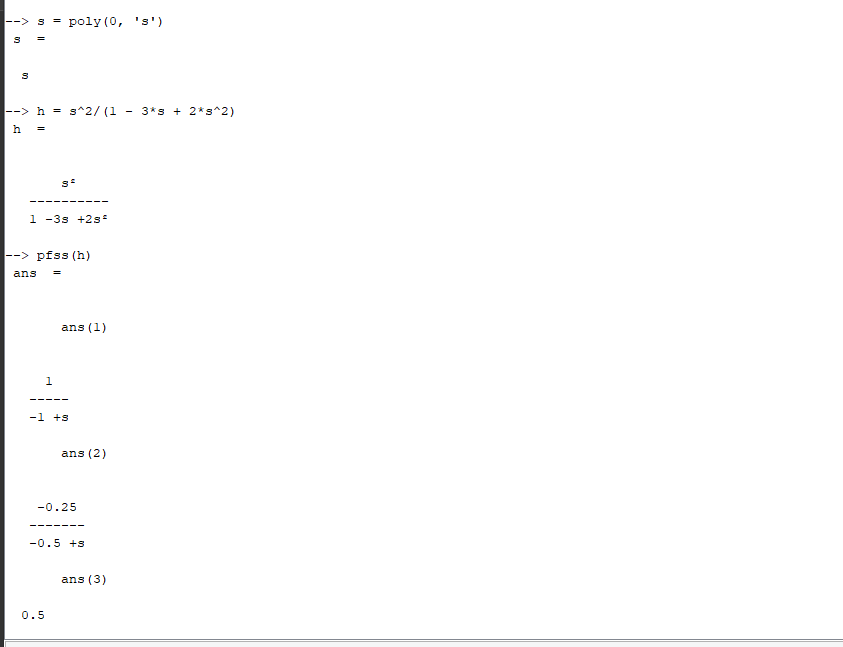
\includegraphics[width=10cm]{cau_a.png}
						\caption{\textit{Code used in Scilab to do partial-fraction expansion}}
					\end{center}
				\end{figure}\\
				$\Rightarrow H(z) = \dfrac{1}{-1 + s} + \dfrac{-0.25}{-0.5 + s} + 0.5 \\
				Replace\ z = s^{-1} \Rightarrow H(z) = \dfrac{1}{-1 + z^{-1}} + \dfrac{-0.25}{-0.5 + z^{-1}} + 0.5 =  \dfrac{-1}{1 - z^{-1}} + \dfrac{0.5}{1 - 2z^{-1}} + 0.5\\ \\
				Result: \left\{\begin{array}{ll}
					h(n) = -u(n) + 0.5 \cdot 2^nu(-n - 1) + 0.5\delta(n),& 1 < |z| < 2 \\
					h(n) = -u(-n - 1) + 0.5 \cdot 2^nu(-n - 1) + 0.5\delta(n),& |z| < 1
				\end{array}\right. \\
				$
			\item $H(z) = \dfrac{z}{z^3 - 6z^2 + 11z - 6}, \qquad |z| < 2$ \\
				$
					\Leftrightarrow H(z) = \dfrac{z^{-2}}{1 - 6z^{-1} + 11z^{-2} - 6z^{-3}} \\
					Replace\ s = z^{-1} \Rightarrow H(s) = \dfrac{s^3}{1 - 6s^1 + 11s^2 -6s^3} \\
				$
				after using Scilab like below:
				\newpage
				\begin{figure}[h!]
					\begin{center}
						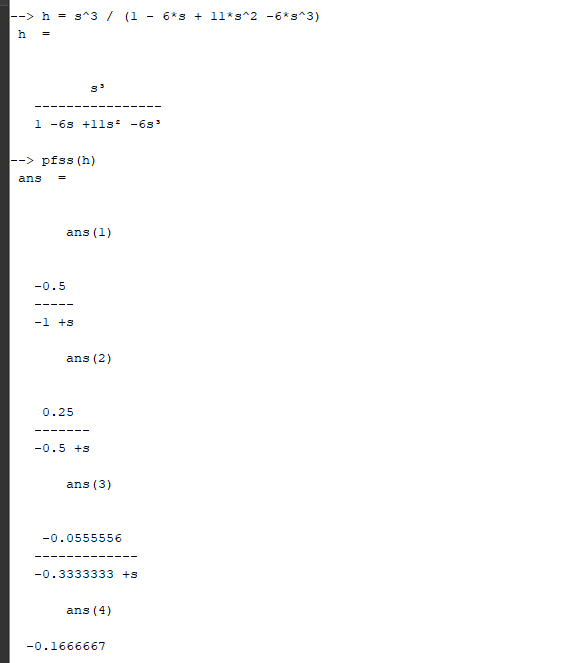
\includegraphics[width=10cm]{cau_b.png}
						\caption{\textit{Code used in Scilab to do partial-fraction expansion}}
					\end{center}
				\end{figure} 
				$
					\Rightarrow H(s) = \dfrac{-0.5}{-1 + s} + \dfrac{0.25}{-0.5 + s} + \dfrac{-\frac{1}{18}}{-\frac{1}{3} + s} + \frac{1}{6} = \dfrac{0.5}{1 - s} + \dfrac{-0.5}{1 - 2s} + \dfrac{\frac{1}{6}}{1 - 3s} + \frac{1}{6} \\
					Replace\ z = s^{-1} \Rightarrow H(z) = \dfrac{0.5}{1 - z^{-1}} + \dfrac{-0.5}{1 - 2z^{-1}} + \dfrac{\frac{1}{6}}{1 - 3z^{-1}} + \frac{1}{6} \\
					Result: \left\{\begin{array}{ll}
						h(n) = 0.5 \cdot u(n) - 0.5 \cdot 2^nu(-n - 1) + \frac{1}{6} \cdot 3^nu(-n - 1) + \frac{1}{6}\delta(n),& 1 < |z| < 2 \\
						h(n) = 0.5 \cdot u(-n - 1) - 0.5 \cdot 2^nu(-n - 1) + \frac{1}{6} \cdot 3^nu(-n - 1) + \frac{1}{6}\delta(n),& |z| < 1
					\end{array}\right. \\
				$
		\end{enumerate}
\end{document}